\newif\ifshowsolutions
\showsolutionstrue
\documentclass{article}
\usepackage{listings}
\usepackage{amsmath}
%\usepackage{subfigure}
\usepackage{subfig}
\usepackage{amsthm}
\usepackage{amsmath}
\usepackage{amssymb}
\usepackage{graphicx}
\usepackage{mdwlist}
\usepackage[colorlinks=true]{hyperref}
\usepackage{geometry}
\usepackage{titlesec}
\geometry{margin=1in}
\geometry{headheight=2in}
\geometry{top=2in}
\usepackage{palatino}
\usepackage{mathrsfs}
\usepackage{fancyhdr}
\usepackage{paralist}
\usepackage{todonotes}
\setlength{\marginparwidth}{2.15cm}
\usepackage{tikz}
\usetikzlibrary{positioning,shapes,backgrounds}
\usepackage{float} % Place figures where you ACTUALLY want it
\usepackage{comment} % a hack to toggle sections
\usepackage{ifthen}
\usepackage{mdframed}
\usepackage{verbatim}
\usepackage[strings]{underscore}
\usepackage{listings}
\usepackage{bbm}
\rhead{}
\lhead{}

\renewcommand{\baselinestretch}{1.15}

% Shortcuts for commonly used operators
\newcommand{\E}{\mathbb{E}}
\newcommand{\Var}{\operatorname{Var}}
\newcommand{\Cov}{\operatorname{Cov}}
\newcommand{\Bias}{\operatorname{Bias}}
\DeclareMathOperator{\argmin}{arg\,min}
\DeclareMathOperator{\argmax}{arg\,max}

% do not number subsection and below
\setcounter{secnumdepth}{1}

% custom format subsection
\titleformat*{\subsection}{\large\bfseries}

% set up the \question shortcut
\newcounter{question}[section]
\newenvironment{question}[1][]
  {\refstepcounter{question}\par\addvspace{1em}\textbf{Question~\Alph{question}\!
    \ifthenelse{\equal{#1}{}}{}{ [#1 points]}: }}
    {\par\vspace{\baselineskip}}

\newcounter{subquestion}[question]
\newenvironment{subquestion}[1][]
  {\refstepcounter{subquestion}\par\medskip\textbf{\roman{subquestion}.\!
    \ifthenelse{\equal{#1}{}}{}{ [#1 points]:}} }
  {\par\addvspace{\baselineskip}}

\titlespacing\section{0pt}{12pt plus 2pt minus 2pt}{0pt plus 2pt minus 2pt}
\titlespacing\subsection{0pt}{12pt plus 4pt minus 2pt}{0pt plus 2pt minus 2pt}
\titlespacing\subsubsection{0pt}{12pt plus 4pt minus 2pt}{0pt plus 2pt minus 2pt}


\newenvironment{hint}[1][]
  {\begin{em}\textbf{Hint: }}{\end{em}}

\ifshowsolutions
  \newenvironment{solution}[1][]
    {\par\medskip \begin{mdframed}\textbf{Solution~\Alph{question}#1:} \begin{em}}
    {\end{em}\medskip\end{mdframed}\medskip}
  \newenvironment{subsolution}[1][]
    {\par\medskip \begin{mdframed}\textbf{Solution~\Alph{question}#1.\roman{subquestion}:} \begin{em}}
    {\end{em}\medskip\end{mdframed}\medskip}
\else
  \excludecomment{solution}
  \excludecomment{subsolution}
\fi

%%%%%%%%%%%%%%%%%%%%%%%%%%%%%%
% HEADER
%%%%%%%%%%%%%%%%%%%%%%%%%%%%%%

\chead{
  {\vbox{
      Machine Learning \& Data Mining \hfill
      Caltech CS/CNS/EE 155 \hfill \\[1pt]
      Miniproject 1\hfill
      February 2024 \\
    }
  }
}

\begin{document}
\pagestyle{fancy}



%%%%%%%%%%%%%%%%%%%%%%%%%%%%%%
% PROBLEM 1
%%%%%%%%%%%%%%%%%%%%%%%%%%%%%%

\newpage

\section{Introduction [15 points]}
    \begin{itemize}
        \item Group members:
        \item Kaggle team name:
        \item Ranking on the private leaderboard:
        \item AUC score on the private leaderboard:
        \item Colab link:
        \item Piazza link:
        \item Division of labor:
    \end{itemize} 
\newpage

\section{Overview [15 points]}
% 1 page maximum
\subsection{Models and techniques attempted}
Fill in

\subsection{Work timeline}
Fill in

\newpage

\section{Approach [20 points]}
% 1 page maximum
\subsection{Data exploration, processing and manipulation}
Fill in

\subsection{Details of models and techniques}
Fill in

\newpage

\section{Model Selection [20 points]}
% 1 page maximum
\subsection{Scoring}
Fill in

\subsection{Validation and test}
Fill in

\newpage

\section{Conclusion [20 points]}
% 1 page maximum
\subsection{Insights}
Fill in

\subsection{Challenges}
Fill in
\newpage

\section{Extra Credit [5 points]}

\newpage

\section{LLM Usage}
This section has an example of LLM usage reporting below. Please follow this format to report LLM usage. Indicate each usage clearly.
\begin{itemize}
    \item Name of LLM(s) Used: ChatGPT
    \item Components of Project involving LLM: Data processing.
\end{itemize}

\subsection{Data preprocessing (example)}

\subsubsection{Interaction (example)}
Only include the parts of the response that you integrated into your project. You may submit screenshots. For example, Figure \ref{fig:llm-output} illustrates the interaction with LLM for data preprocessing. 
Alternatively, you can also write out the prompt and response in text.


\subsubsection{Usage/Integration of Responses (example)}

As shown in Figure~\ref{fig:data-prep-integration}, We used the response as follows, modifying the name of the encoder object and applying it to our training dataframe data, in column some\_column. 

\begin{figure}[htbp]
\centering
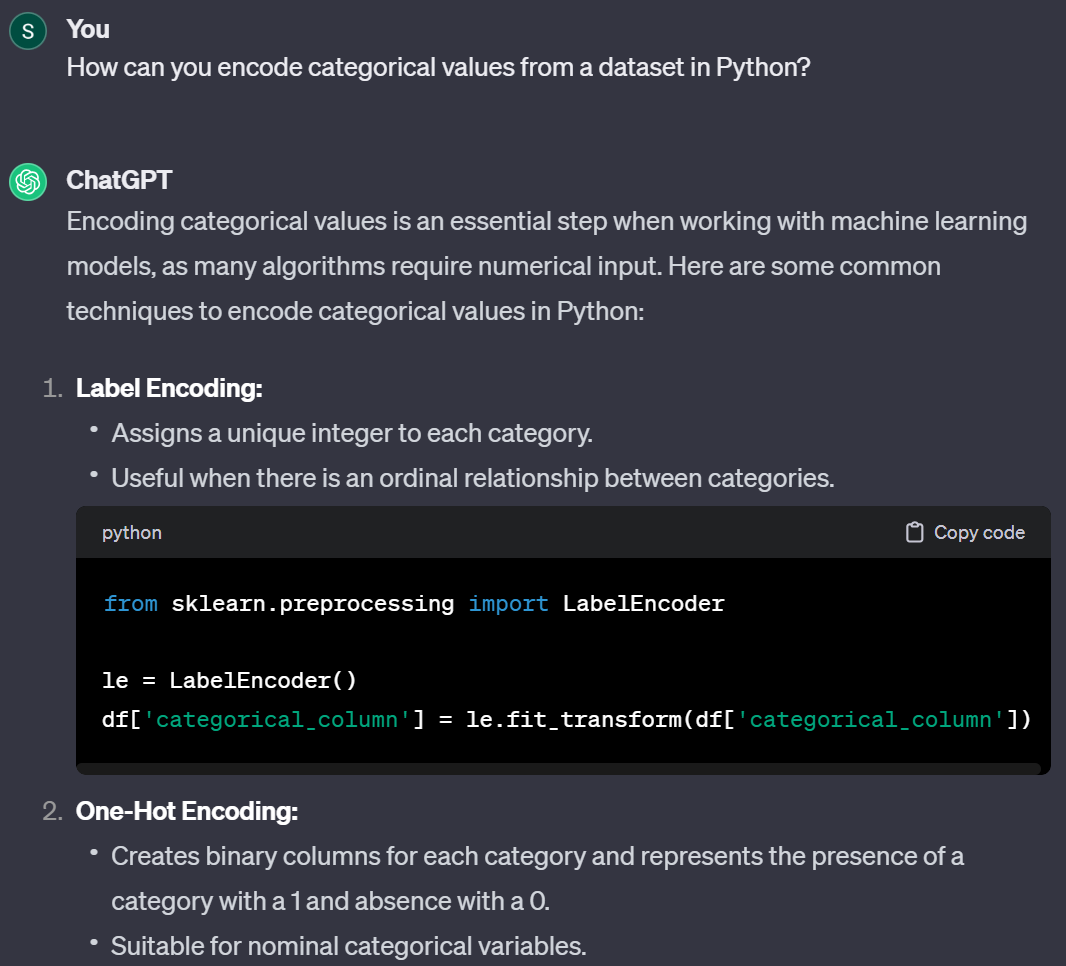
\includegraphics[width=0.68\textwidth]{figs/llm_report_1.png}
    \caption{Interaction with LLM for data preprocessing. }
    \label{fig:llm-output}
\end{figure}

\begin{figure}[t]
    \centering
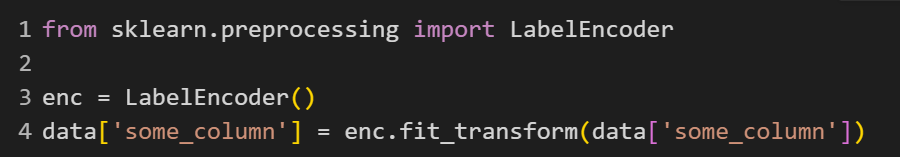
\includegraphics[width=0.68\textwidth]{figs/llm_report_2.png}
    \caption{Integration of LLM's output for data preprocessing}
\label{fig:data-prep-integration}
\end{figure}



\end{document}